\section{Arduino}
Den indledende løsning blev først implementeret på en Arduino Uno mikrocontroller hvorefter konceptet blev testet og verificeret. Koden er derfor i sin indledende fase også skrevet i Arduino.

\begin{figure}[h!]
  \centering
  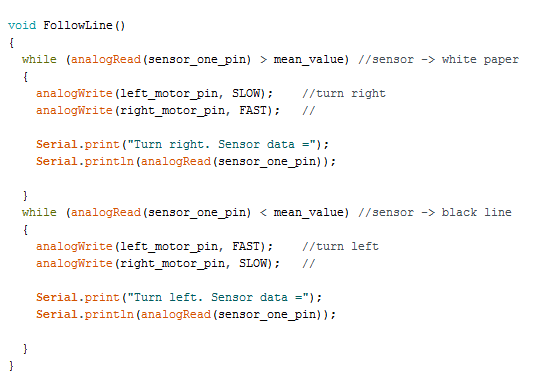
\includegraphics[width=1.0\textwidth]{figures/followLine2.png}
  \caption{FollowLine() funktion.}
  \label{follow_line_kode}
\end{figure}

På overstående figur ses funktionen follow\_Line(). Koden fungerer sålades at når sensoren registrerer den hvide omkringliggende farve drejes der til højre og når den sorte linje registreres drejes der til venstre. Robotten kører derved kun på kanten af linjen. 

\subsection{Test og delkonklussion}
Ud fra det introducerde linetrack system blev konceptet testet ved brug af én sensor på den opstillede bane. 
\newline
Ud fra denne test kan det konkluderes at softwaren virker i henhold til den indledende problemløsning. Robotten er i stand til at følge kanten af linjen ved hjælp af de forskellige overfladefarveværdier som sensoren registrerede gennem testen. 
\newline

\begin{figure}[h!]
  \centering
  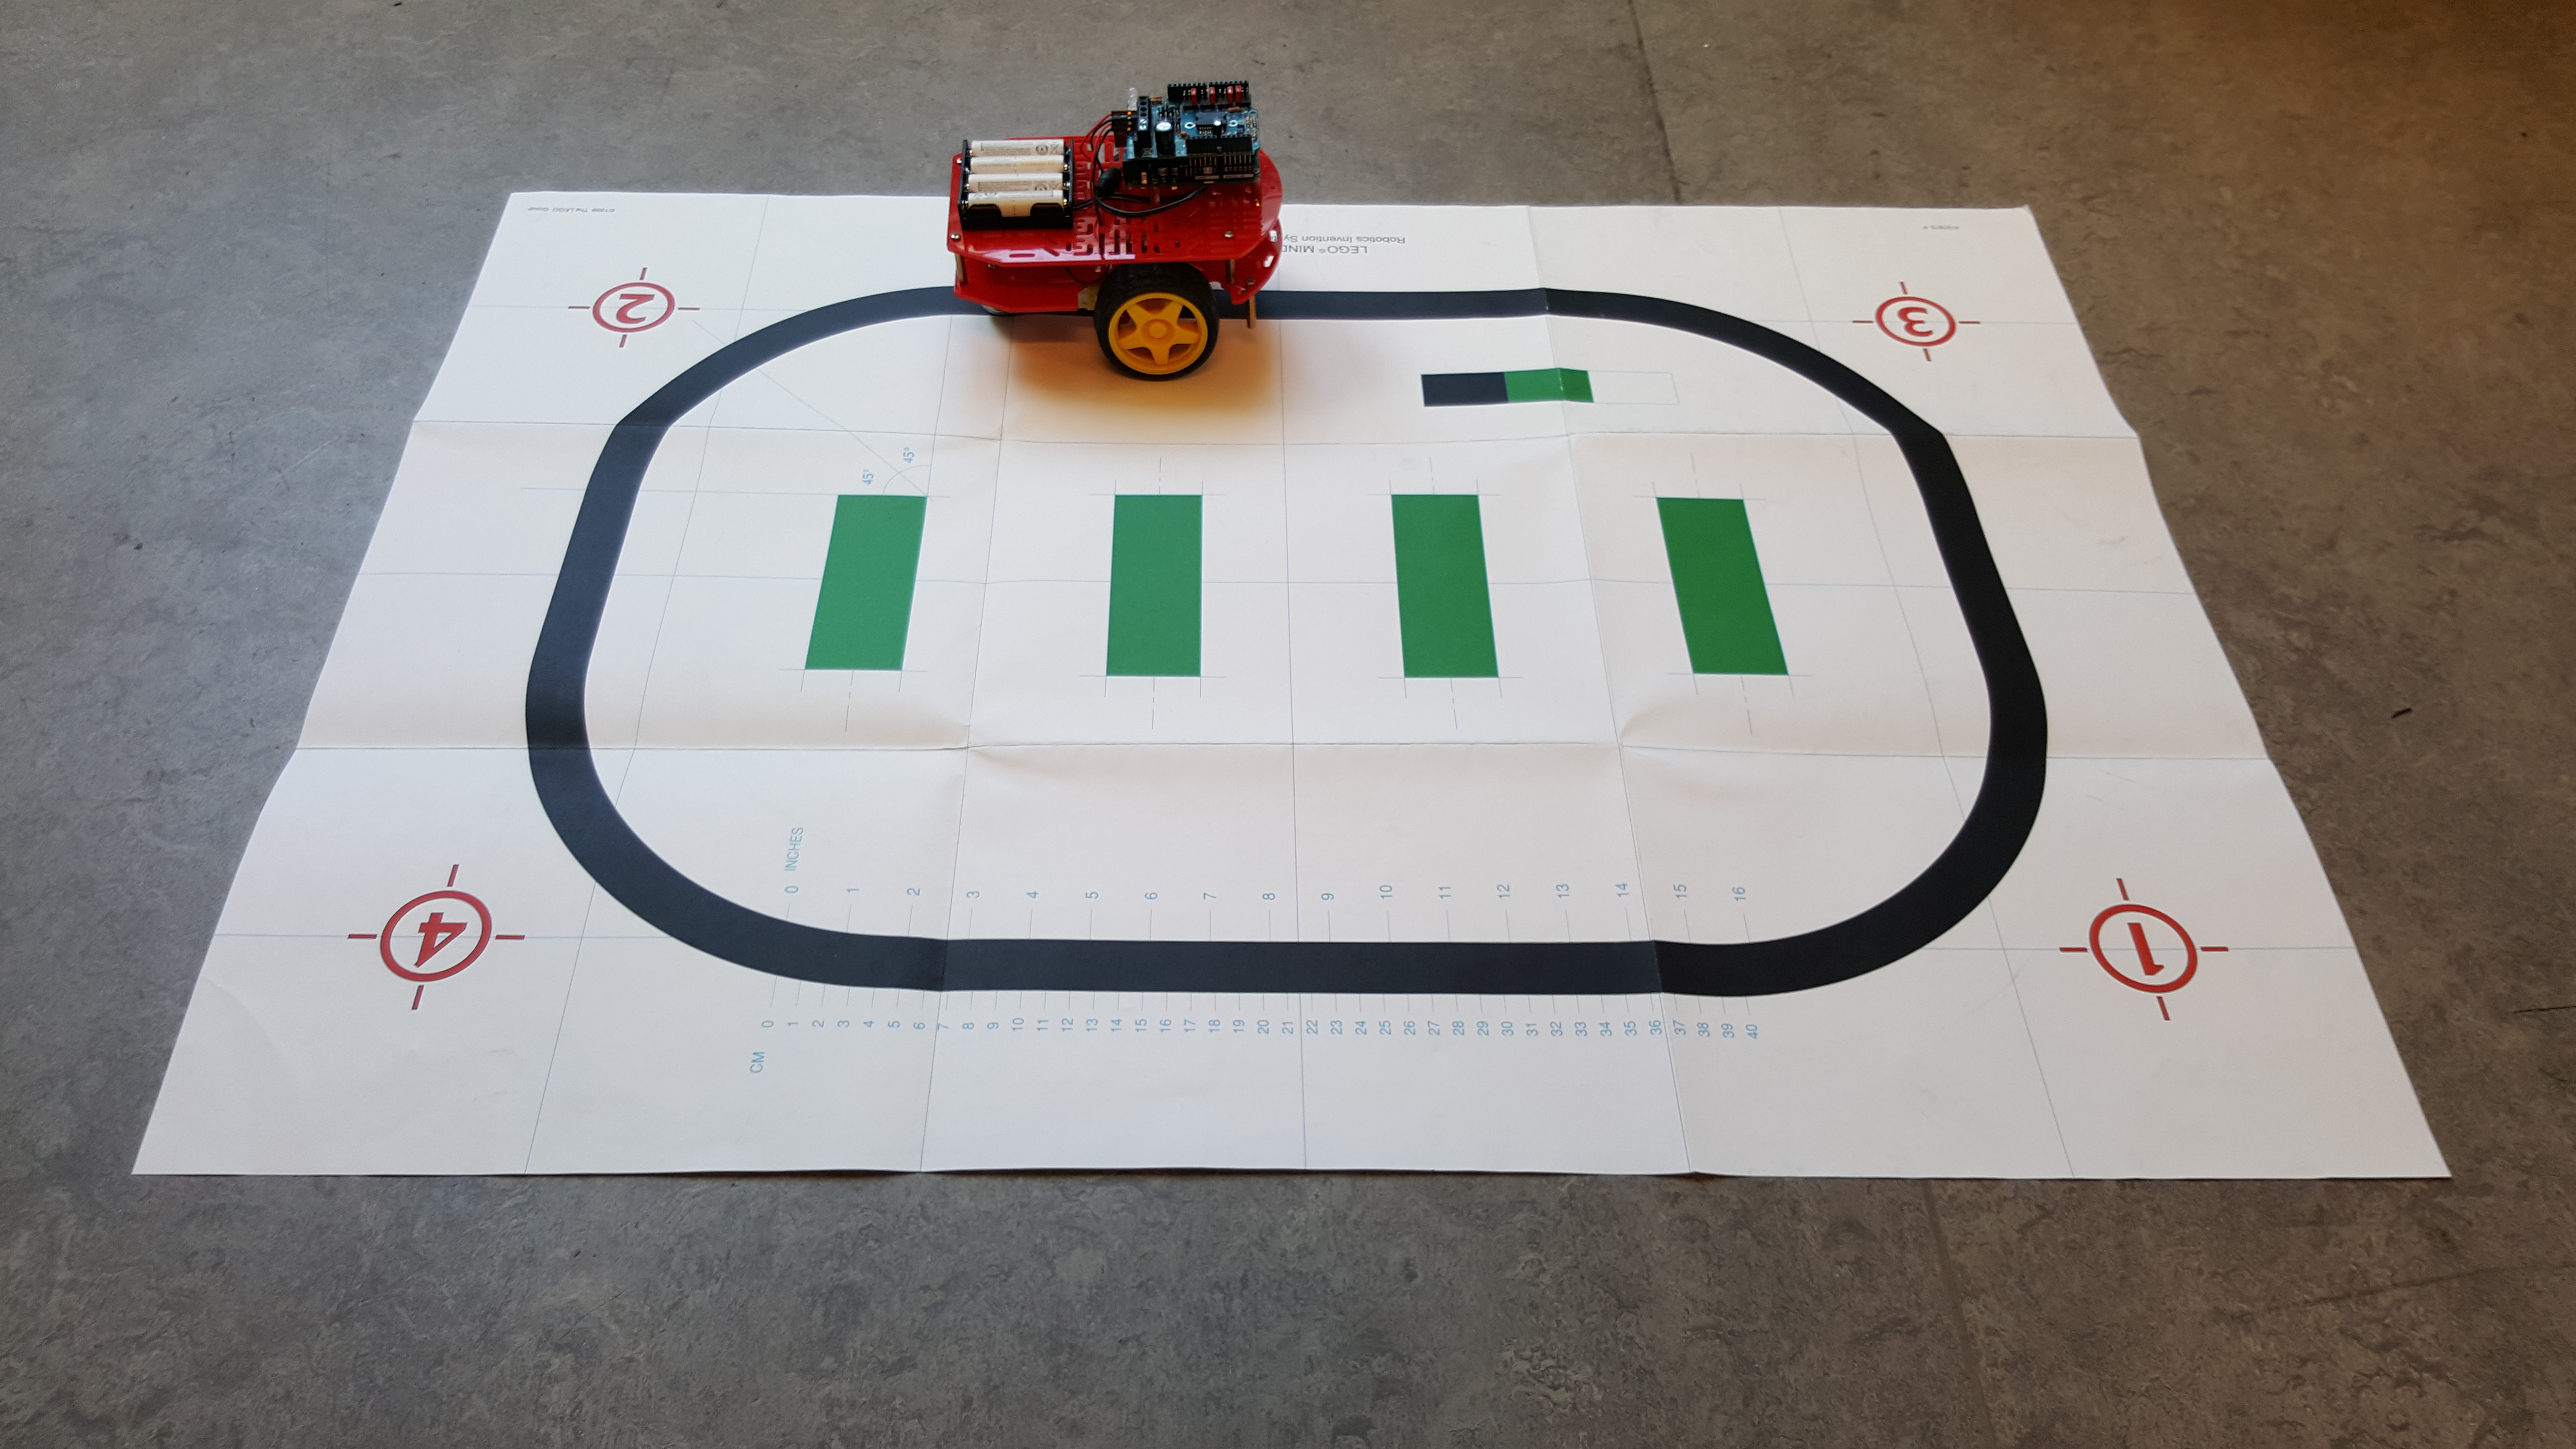
\includegraphics[width=0.6\textwidth]{figures/testMedEnSensor.png}
  \caption{Den inledende software løsning til linetrackinging med 1 sensor i et superloop.}
  \label{indledende_test}
\end{figure}

\subsection*{Implementering af flere sensore}
For at robotten er i stand til at kunne følge linjen hurtigst og bedst muligt implementeres ydereligere sensore. Dette gøres for at robotten kan navigere nøjagtigt og præcist. Sensorene er placeret ud fra en skabelon som gruppen har 3D printet for at skabe de bedste omstændigheder muligt for at få så præcise måliner som muligt.
\newline 
Her anvendes konceptet vist i figur \ref{line_track} i Line Track. \fxnote{lav reference til line track}. Herfra ændres softwaren fra den indledende problemløsning nu til at håndtere tre sensore i stedet for én. 

\begin{figure}[h!]
  \centering
  \includegraphics[width=0.5\textwidth]{figures/lineTrackingFlowchartMultibleSensors.png}
  \caption{Software flowchart over problemløsningen ved hjælp af tre sensore i et superloop.}
  \label{flowchart_flere_sensorer}
\end{figure}

Som det ses i overstående figur ses de fire mulige scenarier som er præsenteret i Line Track. \fxnote{reference til line track}
Som vist i flowchartet registrerer sensorene om stregen er visuel for sensoren eller ej. Såfremt sensoren registrerer en værdi som fortæller om den er på stregen, kører robotten ligeud indtil en anden værdi måles. 
\newline 
Hvis en anden sensor end den midterste afgiver en måling af den opstillede bane angiver dette at banens forløb har ændret sig, og robotten anvender derved de to funktioner anvist i flowchartet hvorvidt der skal justeres til venstre eller højre. 
\newline
Såfremt ingen fejlmålinger fra sensoren eller svans stopper robotten fortsætter denne i et superloop.

\subsubsection{Videreudvikling af Arduino kode}
\begin{figure}[h!]
  \centering
  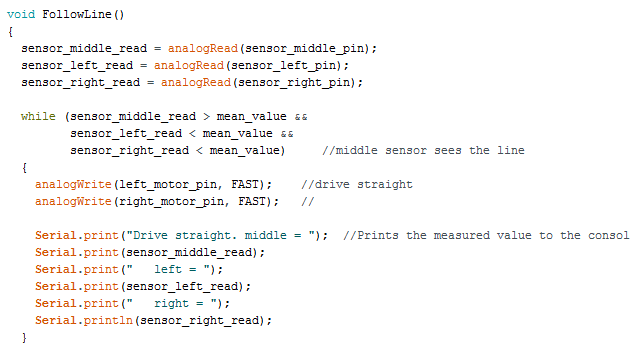
\includegraphics[width=1.0\textwidth]{figures/treSensoreFollowLine.png}
  \caption{Software flowchart over problemløsningen ved hjælp af tre sensore i et superloop.}
  \label{tre_sensore_followline}
\end{figure}

\fxnote {indsæt her billede af koden med tre sensorer}

 

